% Template for ICIP-2018 paper; to be used with:
%          spconf.sty  - ICASSP/ICIP LaTeX style file, and
%          IEEEbib.bst - IEEE bibliography style file.
% --------------------------------------------------------------------------
\documentclass{article}
\usepackage{spconf,amsmath,graphicx,url}

% Example definitions.
% --------------------
\def\x{{\mathbf x}}
\def\L{{\cal L}}

% Title.
% ------
\title{REAL-TIME TRASHCAN RECOGNIZER AND LOCALIZER FOR THE BLIND AND VISUALLY IMPAIRED}
%
% Single address.
% ---------------
\name{A. Abuyazid, A. Shukla, M. Swaminathan\thanks{Thanks to Dr. Alan C Bovik, Cockrell Family Regents Endowed Chair Professor, The University of Texas at Austin}}
%
% For example:
% ------------
\address{The University of Texas at Austin\\
	Department of Electrical and Computer Engineering\\
	Austin, TX 78712 USA}
%
% Two addresses (uncomment and modify for two-address case).
% ----------------------------------------------------------
%\twoauthors
%  {A. Author-one, B. Author-two\sthanks{Thanks to XYZ agency for funding.}}
%	{School A-B\\
%	Department A-B\\
%	Address A-B}
%  {C. Author-three, D. Author-four\sthanks{The fourth author performed the work
%	while at ...}}
%	{School C-D\\
%	Department C-D\\
%	Address C-D}
%
\begin{document}
%\ninept
%
\maketitle
%
\begin{abstract}
With 324 million people blind and visually impaired in the world and the cane still being the primary assistive device used, we approached this problem by looking at it through a different lens. Quite literally a lens. Through involvement with the National Federation of the Blind, we learned that trivial tasks such as finding a public trash can is almost impossible with merely a cane. Using cameras to help the blind is a pre-existing domain, however, we decided to attack this subproblem of navigating the user to public trash cans. Although seemingly trivial, this concept can be expanded to solve larger, problems such as steering the blind away from hazardous construction, reading signs, and perhaps one day driving (unless self driving cars are prominent by then).
\end{abstract}
%
\begin{keywords}
Image processing, object detection, assistive technology
\end{keywords}
%
\section{INTRODUCTION}
\label{sec:intro}

We have developed a wearable device to assist blind people in navigation, specifically in finding public trash cans. The device identifies and detects the position of nearby trash cans using an Intel Realsense camera and provides vibrational feedback via a wrist band controlled by a RaspberryPi 3 to indicate this location to the wearer. The software for localizing the trash cans employs image processing algorithms in combination with machine learning and has been developed in Python. Although this device is only a starting point, the project could be extended to detect many other objects.

\section{RELATED WORK}
\label{sec:research}
Several tools to assist the visually impaired in navigation using computer vision have been developed. 
A project from Stanford called ‘Let Blind People See’ detects objects and converts their position into 3D sound to help blind people locate them~\cite{LetBlind}.

Another study uses vibrational feedback similar to that used our device to help the visually impaired avoid obstacles~\cite{Kinect}. This study indicated that haptic feedback at the wrist is one of the most effective methods of guidance for the blind.

These projects guided the development of our device, which includes elements of both, localizing a specific object and providing haptic feedback for guidance.

\section{PROCESS}
\label{sec:theprocess}

Here we go through the process we used for crafting this device. We begin with discussing about the camera, frame processing and model, and conclude with the physical device.

\subsection{REALSENSE CAMERA}
\label{ssec:realsense}

For this device, we used an Intel Realsense D435 camera to use to detect the trash cans. We chose this because of its relatively small size and since it had two lenses that we could extrapolate depth from. The camera also had depth sensing capabilities, but we chose not to use that and instead use triangulation properties to infer depth because if this device were to become an actual product, the cost of obtaining a camera with depth capabilities are significantly more expensive than using two cameras side by side. The horizontal FOV (field of vision) for the Realsense camera is 86 degrees and the vertical is 57 degrees. We used the librealsense python interface \cite{realsense} to capture the individual frames to use for processing. We did not have the capabilities to change the frame of the camera, but we instead modulated the rate at which we sampled the frame in software. 

\subsection{FRAME PRE-PROCESSING}
\label{ssec:frprep}

Ultimately, this device is supposed to be a wearable device, and we kept that in mind as we determined the frame image pre-processing. From training our model, discussed in the model section, we realized that we did not need such a high resolution for the model to work and detect the trash can, so we experimented with downsampling amounts, given by the following forrmula, $J(i) = I(Li)]$ \cite{Bovik19}, where L is the downsampling rate. We used OpenCV \cite{opencv_library} to specify the end dimensions instead of L. We found that we could donwsample the image as much as half its dimensions, or $L = 2$ and the model still worked just as well. This also helped the latency of the device. Refer to \textbf{Fig 1.} to see difference in images. 

\subsection{DATA PRUNING AND CONNECTED COMPONENT LABELING}
\label{ssec:dataprune}

Since the portion of ImageNet that corresponded with trash can images was under maintenence as we were unable to access it, the ADE20K \cite{zhou2017scene}, was a dataset that we found that fulfilled our purpose. It contained images with prer-segmented components corresponding to object classes. We took the images with trash cans and counted the number of trash cans in an image using conected component labeling, and used the fully connected component to draw a bounding box around the trash cans. We then overlayed the coordinated of this bounding box on the original image to feed into our model. 

\subsection{THE MODEL}
\label{ssec:themodel}
We used a platform called Gluon \cite{gluoncvnlp2019} that allowed us to create a transfer learning model to learn the trash cans. 
We used an efficient model designed specifically for mobile and embedded vision applications called efficient MobileNet, that had been pretrained on the VOC database using Single Shot MultiBox Detector (SSD) algorithm\cite{Howard2017MobileNetsEC,Liu2016SSDSS} to learn the trash cans. 
Since we did not need all the object classes, we morphed this MobileNet neural network into a binary classifier by having it output only whether the object was a trash can or not.
A future method for this could be to train our own classifier instead of using transfer learning or eliminating the last several layers of a deep network and appending a boosting, support vector machine, etc. classifier since this method will save memory by eliminating the deep layers that learn other object classes. 

\subsection{BOOSTING ACCURACY VIA POST TRAINING IMAGE PROCESSING}
\label{ssec:boosting}

As we trained the model on our trash can images, we noticed that there was not a very high confidence value given to a trash can and the model generalized dark rectangular objects as trash cans when they were not. To account for this, since we had limited data as well, we used several image processing techniques to feed in better images into the network. We experimented with several prssibilities and combinations, including edge filtering and Felsenszwalb's graph based image segmentation to boost edges, and ended up chosing a combination of median filtering and erosion with a crosshair kernel on the image. The intuition behind using a median filter was that it denoised the image enough so that it eliminated noise but maintained the edge details of the trash cans. The erosion was used because the Realsense produced small white dots that were distorting the image slightly. 

\begin{center}
\begin{figure}
%
\begin{minipage}[b]{.48\linewidth}
  \centering
  \centerline{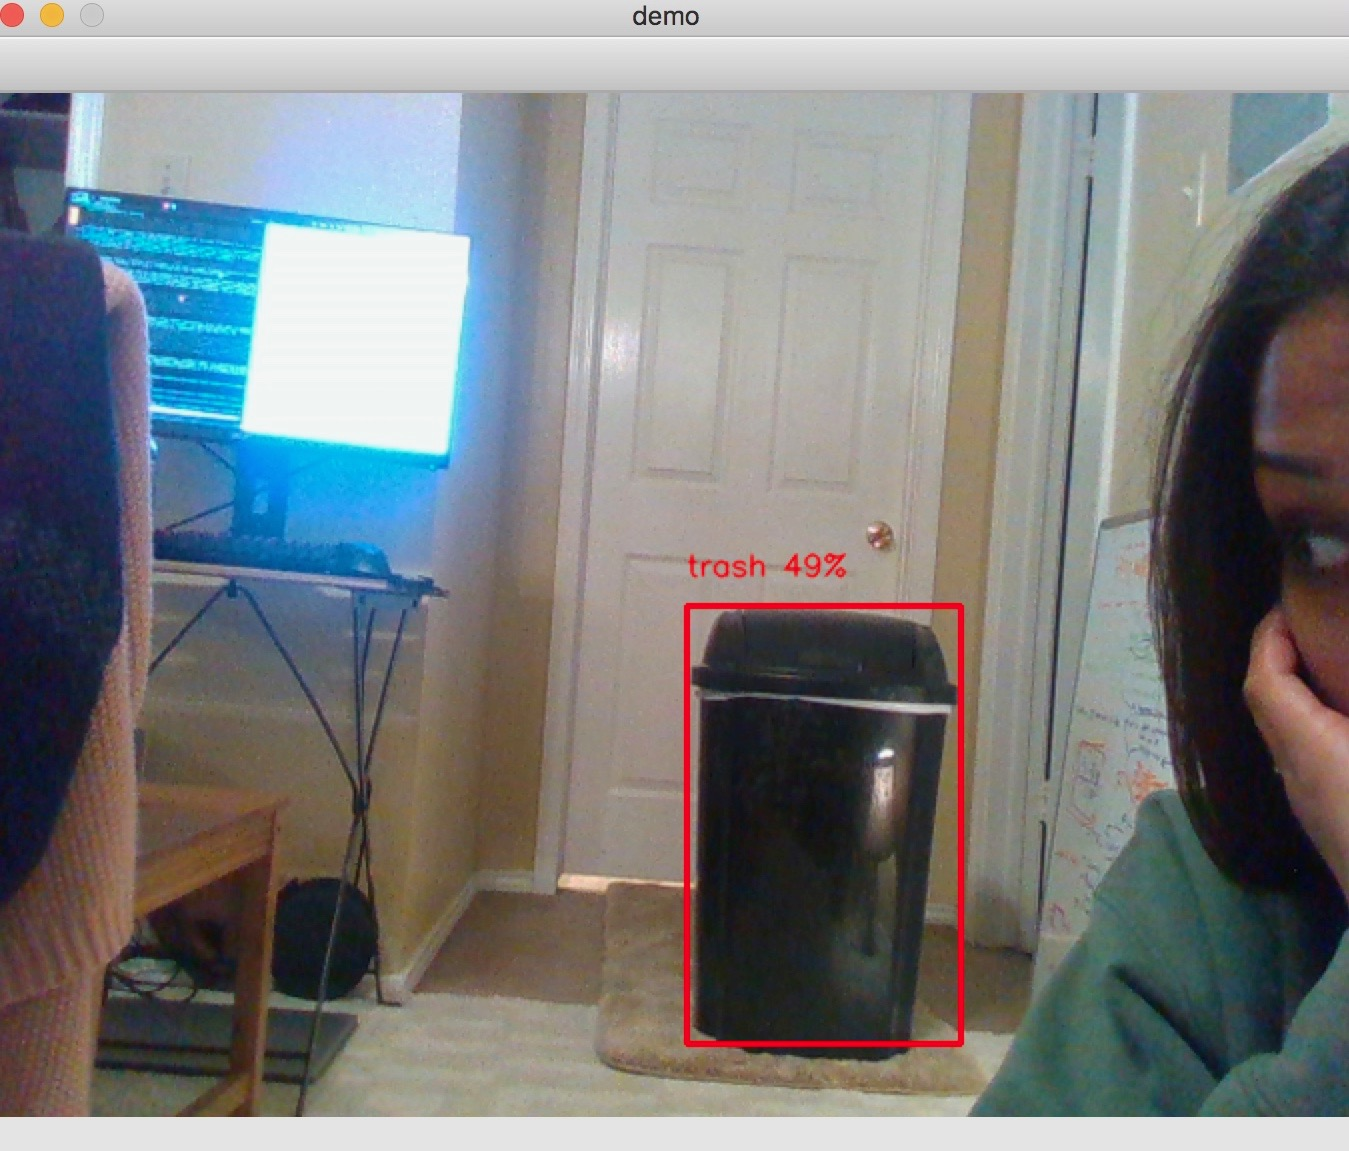
\includegraphics[width=4.0cm]{fullres.jpg}}
%  \vspace{1.5cm}
  \centerline{(a) No downsample, unprocessed}\medskip
\end{minipage}
\hfill
\begin{minipage}[b]{0.48\linewidth}
  \centering
  \centerline{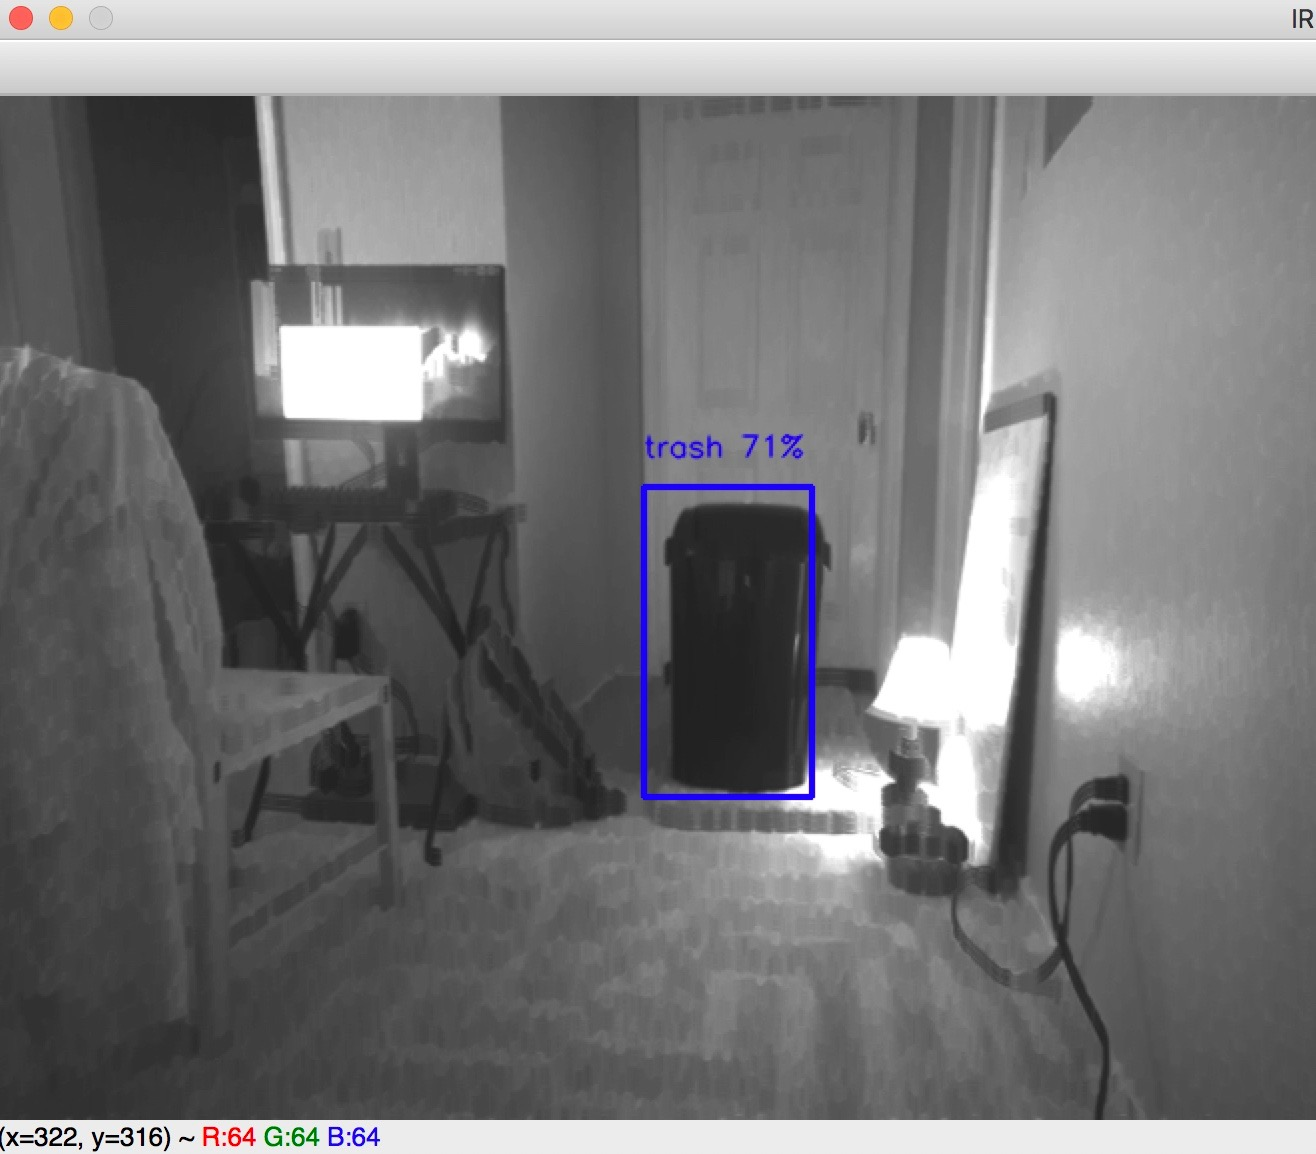
\includegraphics[width=4.0cm]{processed.jpg}}
%  \vspace{1.5cm}
  \centerline{(b) Downsample, processed}\medskip
\end{minipage}
%
\caption{Disparity in model confidence between pure and processed frames.}
\label{figures2}
%
\end{figure}
\end{center}




\subsection{BINOCULAR CAMERA GEOMETRY AND TRIANGULATION FOR DEPTH APPROXIMATION}
\label{ssec:triangulation}

In order to get an approximate depth measurement to notify the user how far away the trash can is, we used binocular camera geometry and triangulation properties. We first took the horizontal disparity betwwen the images, the lens focal lengths, and the distance between the two stereoscopic lenses. Next we used the triangulation equation, $Z_0 = \frac{2Df}{dx}$ \cite{Bovik19} to approximate the depth Z. We had to do some calibration (in essence, multiply by sclars and then project the results in the [0,9] interval for the embedded systems component) to get the depth to work. We then cross referenced this with the percentage of the y-axis component of the bounding box with the total height of the frame to make sure that our triangulation equation was working approximately well. 

\subsection{THE DEVICE}
\label{ssec:thedevice}

The device is in the form of a wrist band that contains a 2-dimensional array of haptic motors to relay angular position and distance feedback to the user corresponding to the found trash can. The corresponding LED grid was only for demo purposes so that the audience can view which haptic motors are being activated. We decided on a wrist cuff since the study from the paper, Guiding Blind People with Haptic Feedback, found that the wrist and spine were the best places to detect vibrational impulses \cite{guiding_blind}. In their study they used 2 wristbands, but we decided to go with one wristband representing 86 degrees since this was the horizontal FOV (field of vision) of the Intel Realsense camera. We used a RaspberryPi 3 to control the device and to communicate with the camera, we used a wireless TCP protocol.

% Below is an example of how to insert images. Delete the ``\vspace'' line,
% uncomment the preceding line ``\centerline...'' and replace ``imageX.ps''
% with a suitable PostScript file name.
% -------------------------------------------------------------------------
\begin{center}
\begin{figure}[ht]

\begin{minipage}[b]{1.0\linewidth}
  \centering
  \centerline{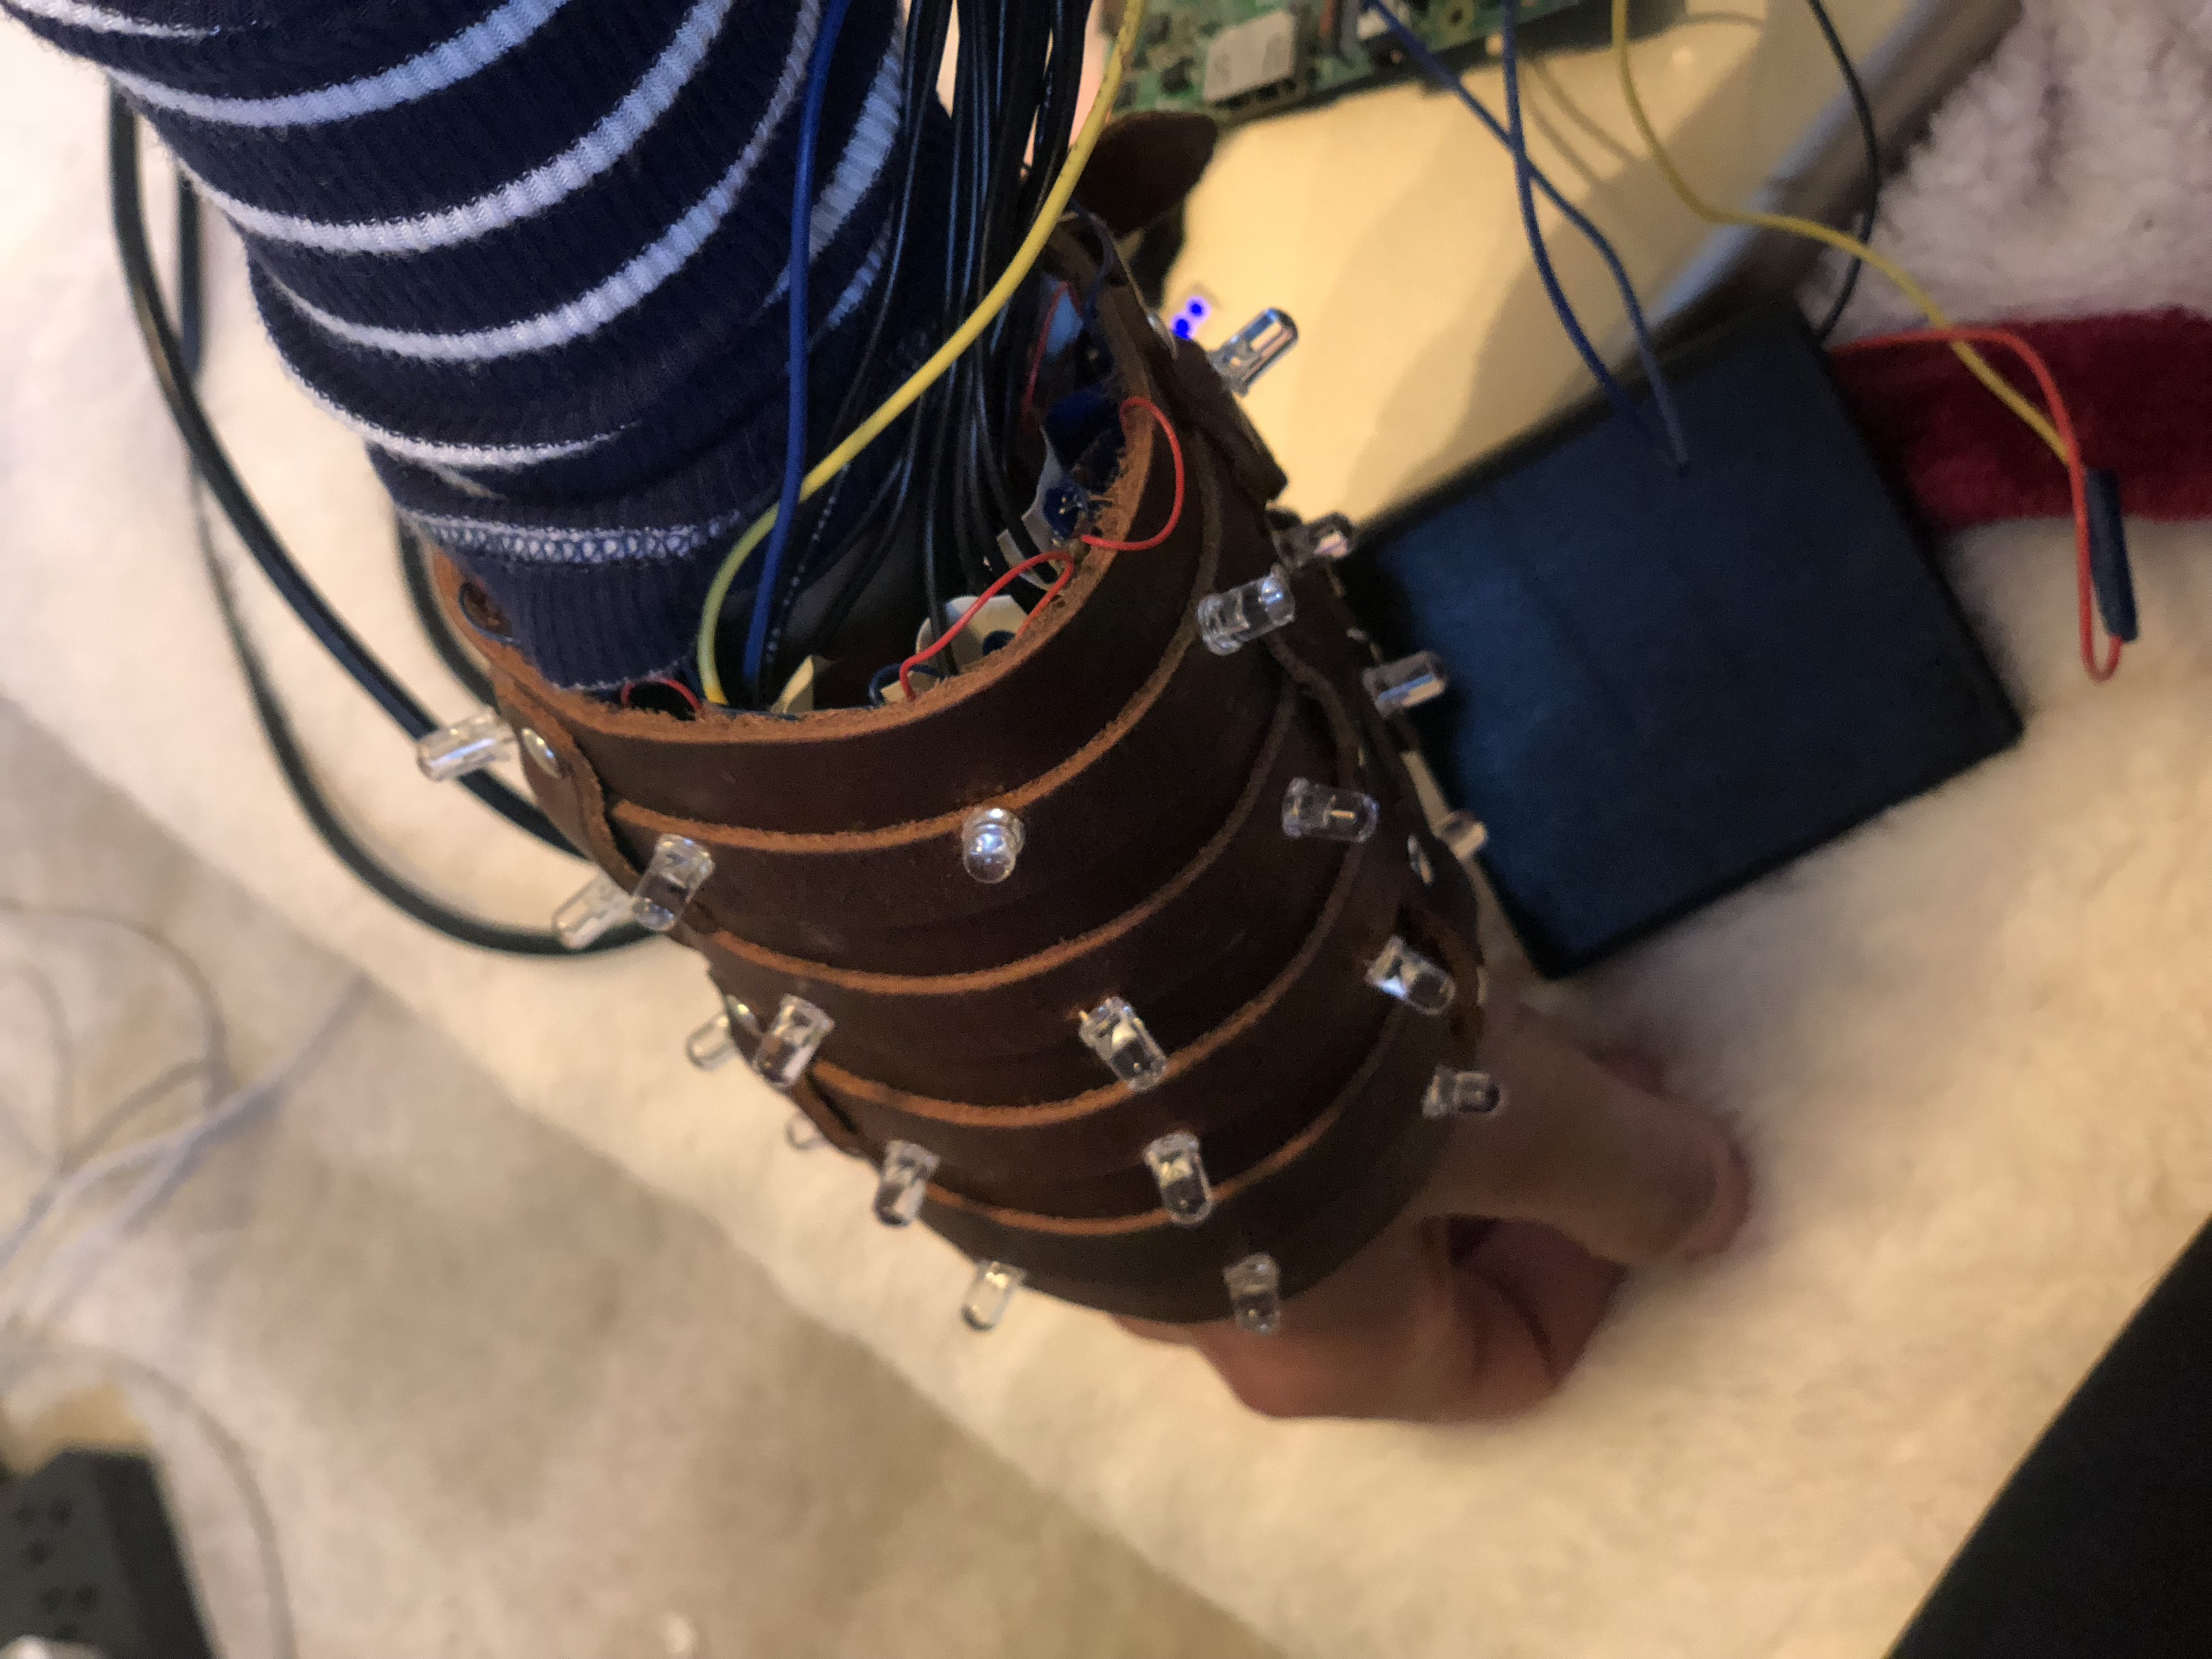
\includegraphics[width=8.5cm]{worn.JPG}}
%  \vspace{2.0cm}
  \centerline{(a) Device worn on wrist}\medskip
\end{minipage}
%
\begin{minipage}[b]{.48\linewidth}
  \centering
  \centerline{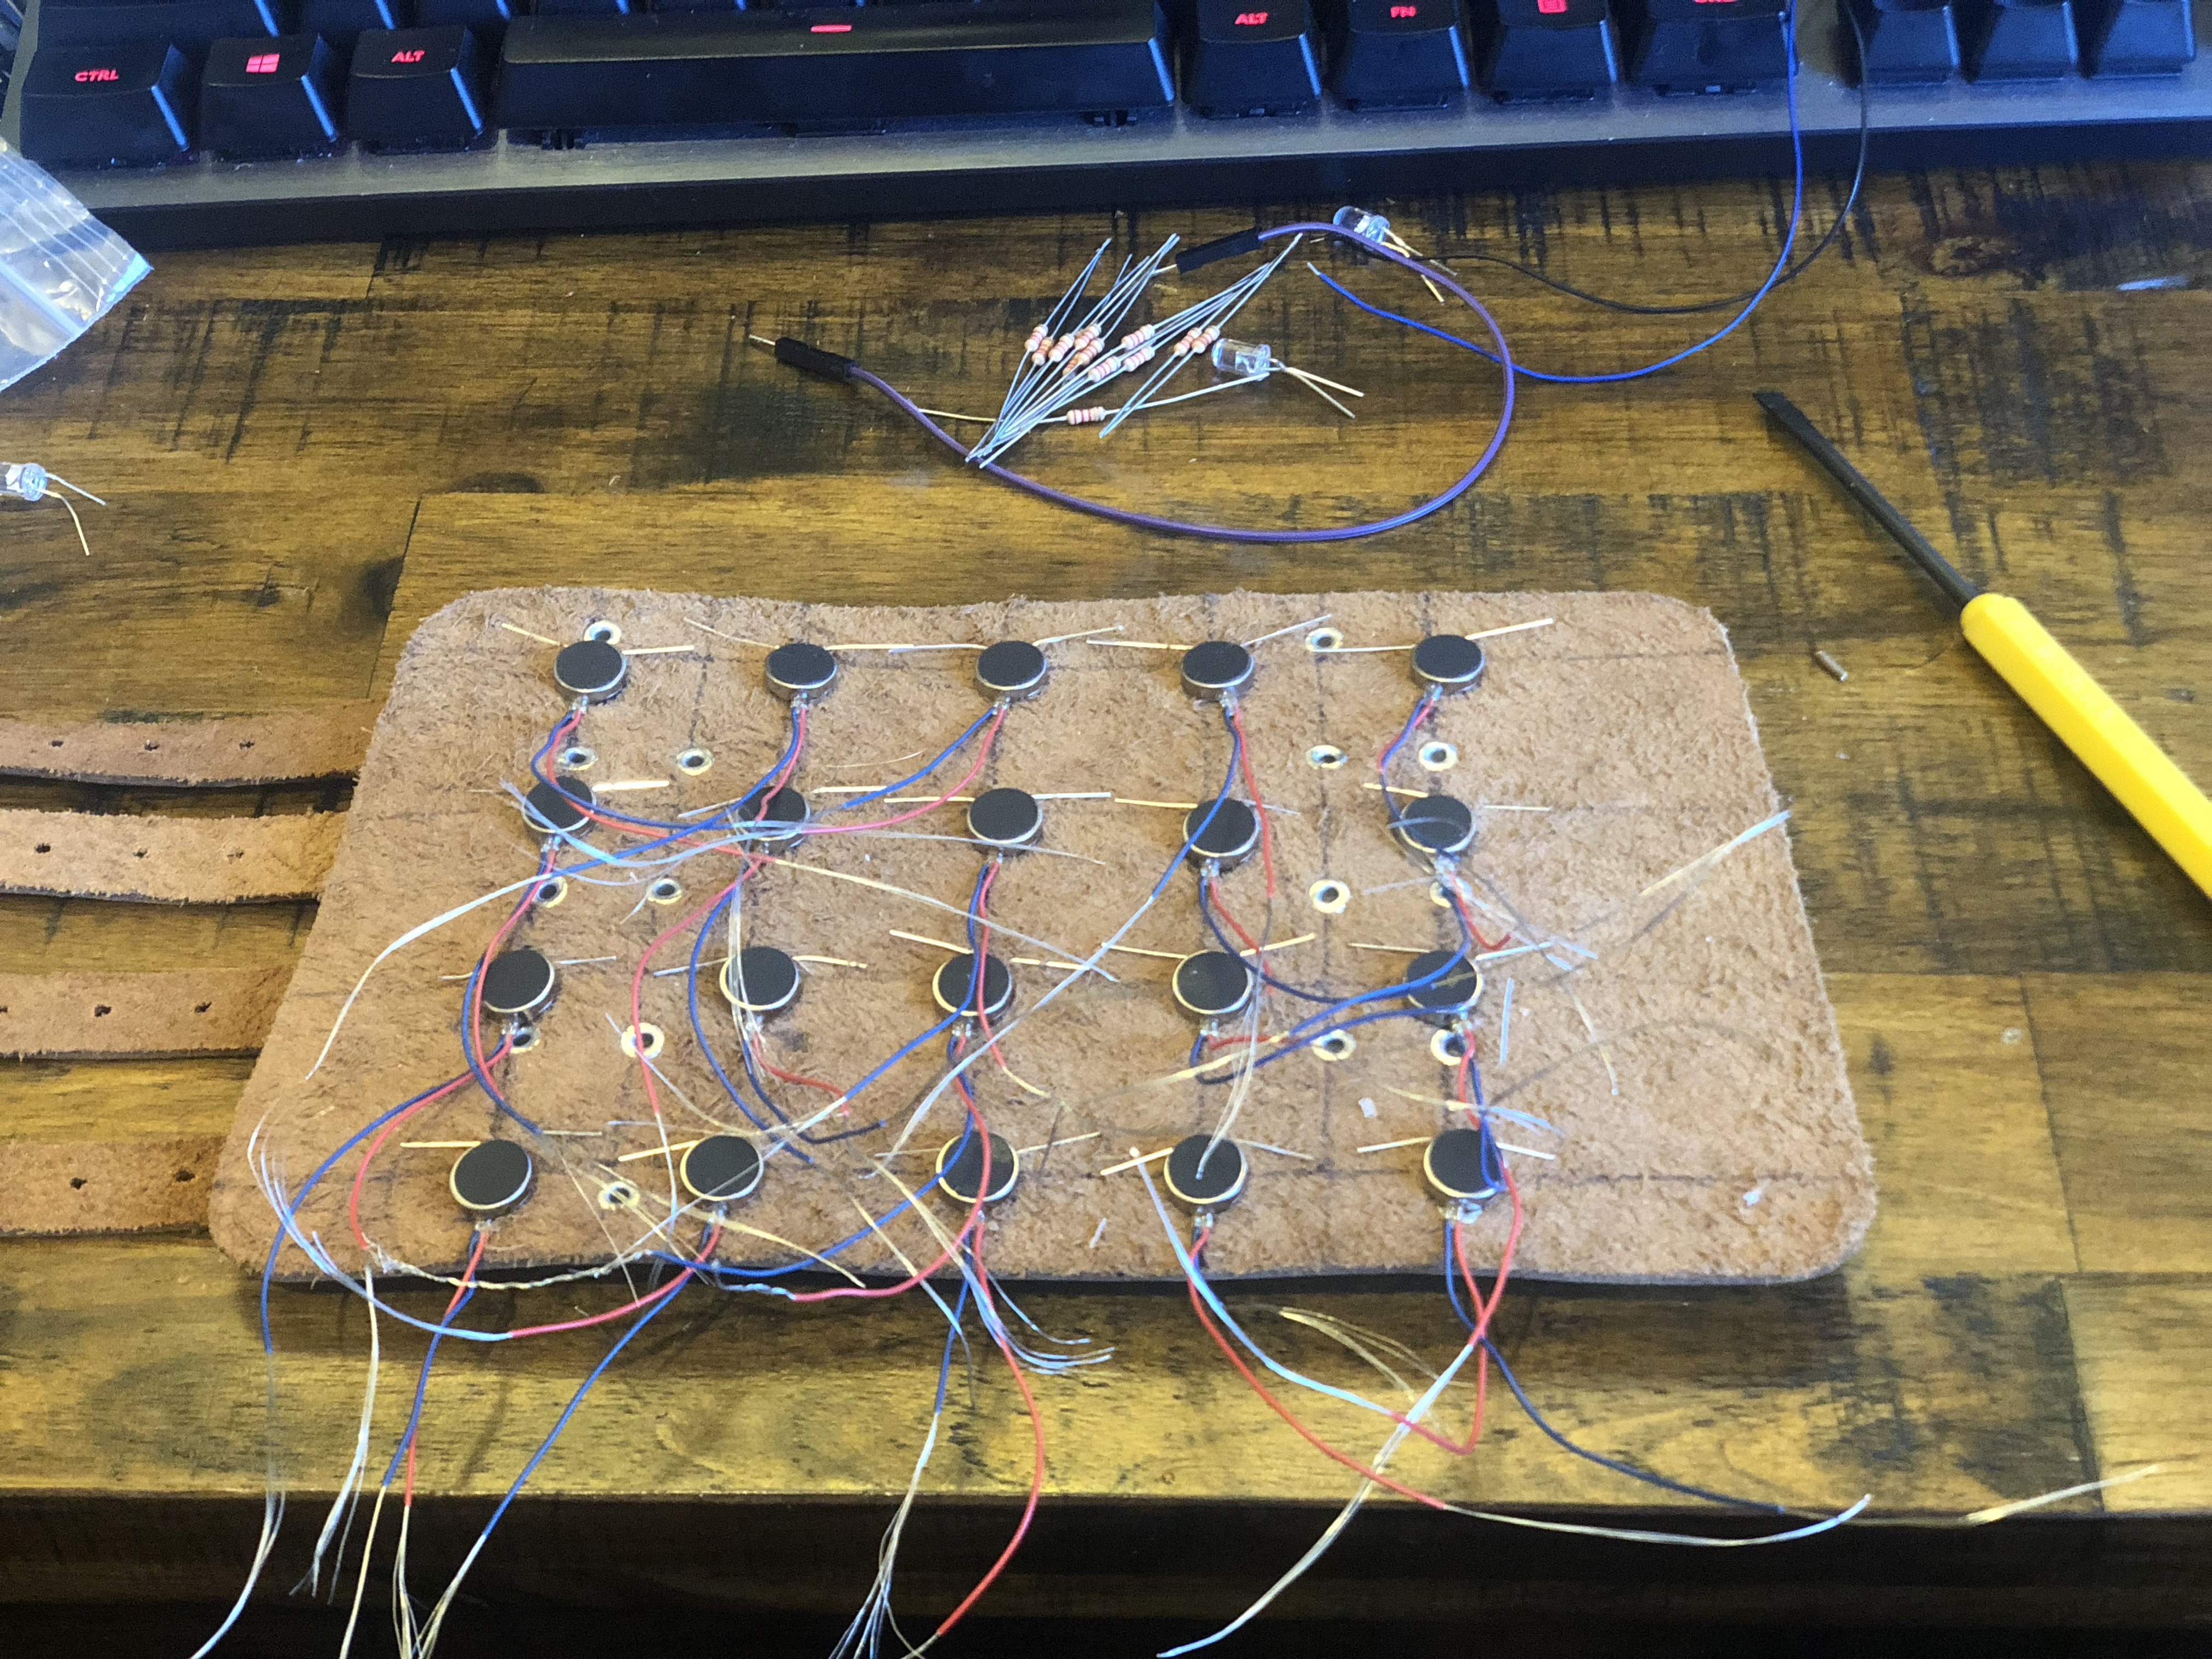
\includegraphics[width=4.0cm]{hapticmotors.JPG}}
%  \vspace{1.5cm}
  \centerline{(b) Haptic motor grid}\medskip
\end{minipage}
\hfill
\begin{minipage}[b]{0.48\linewidth}
  \centering
  \centerline{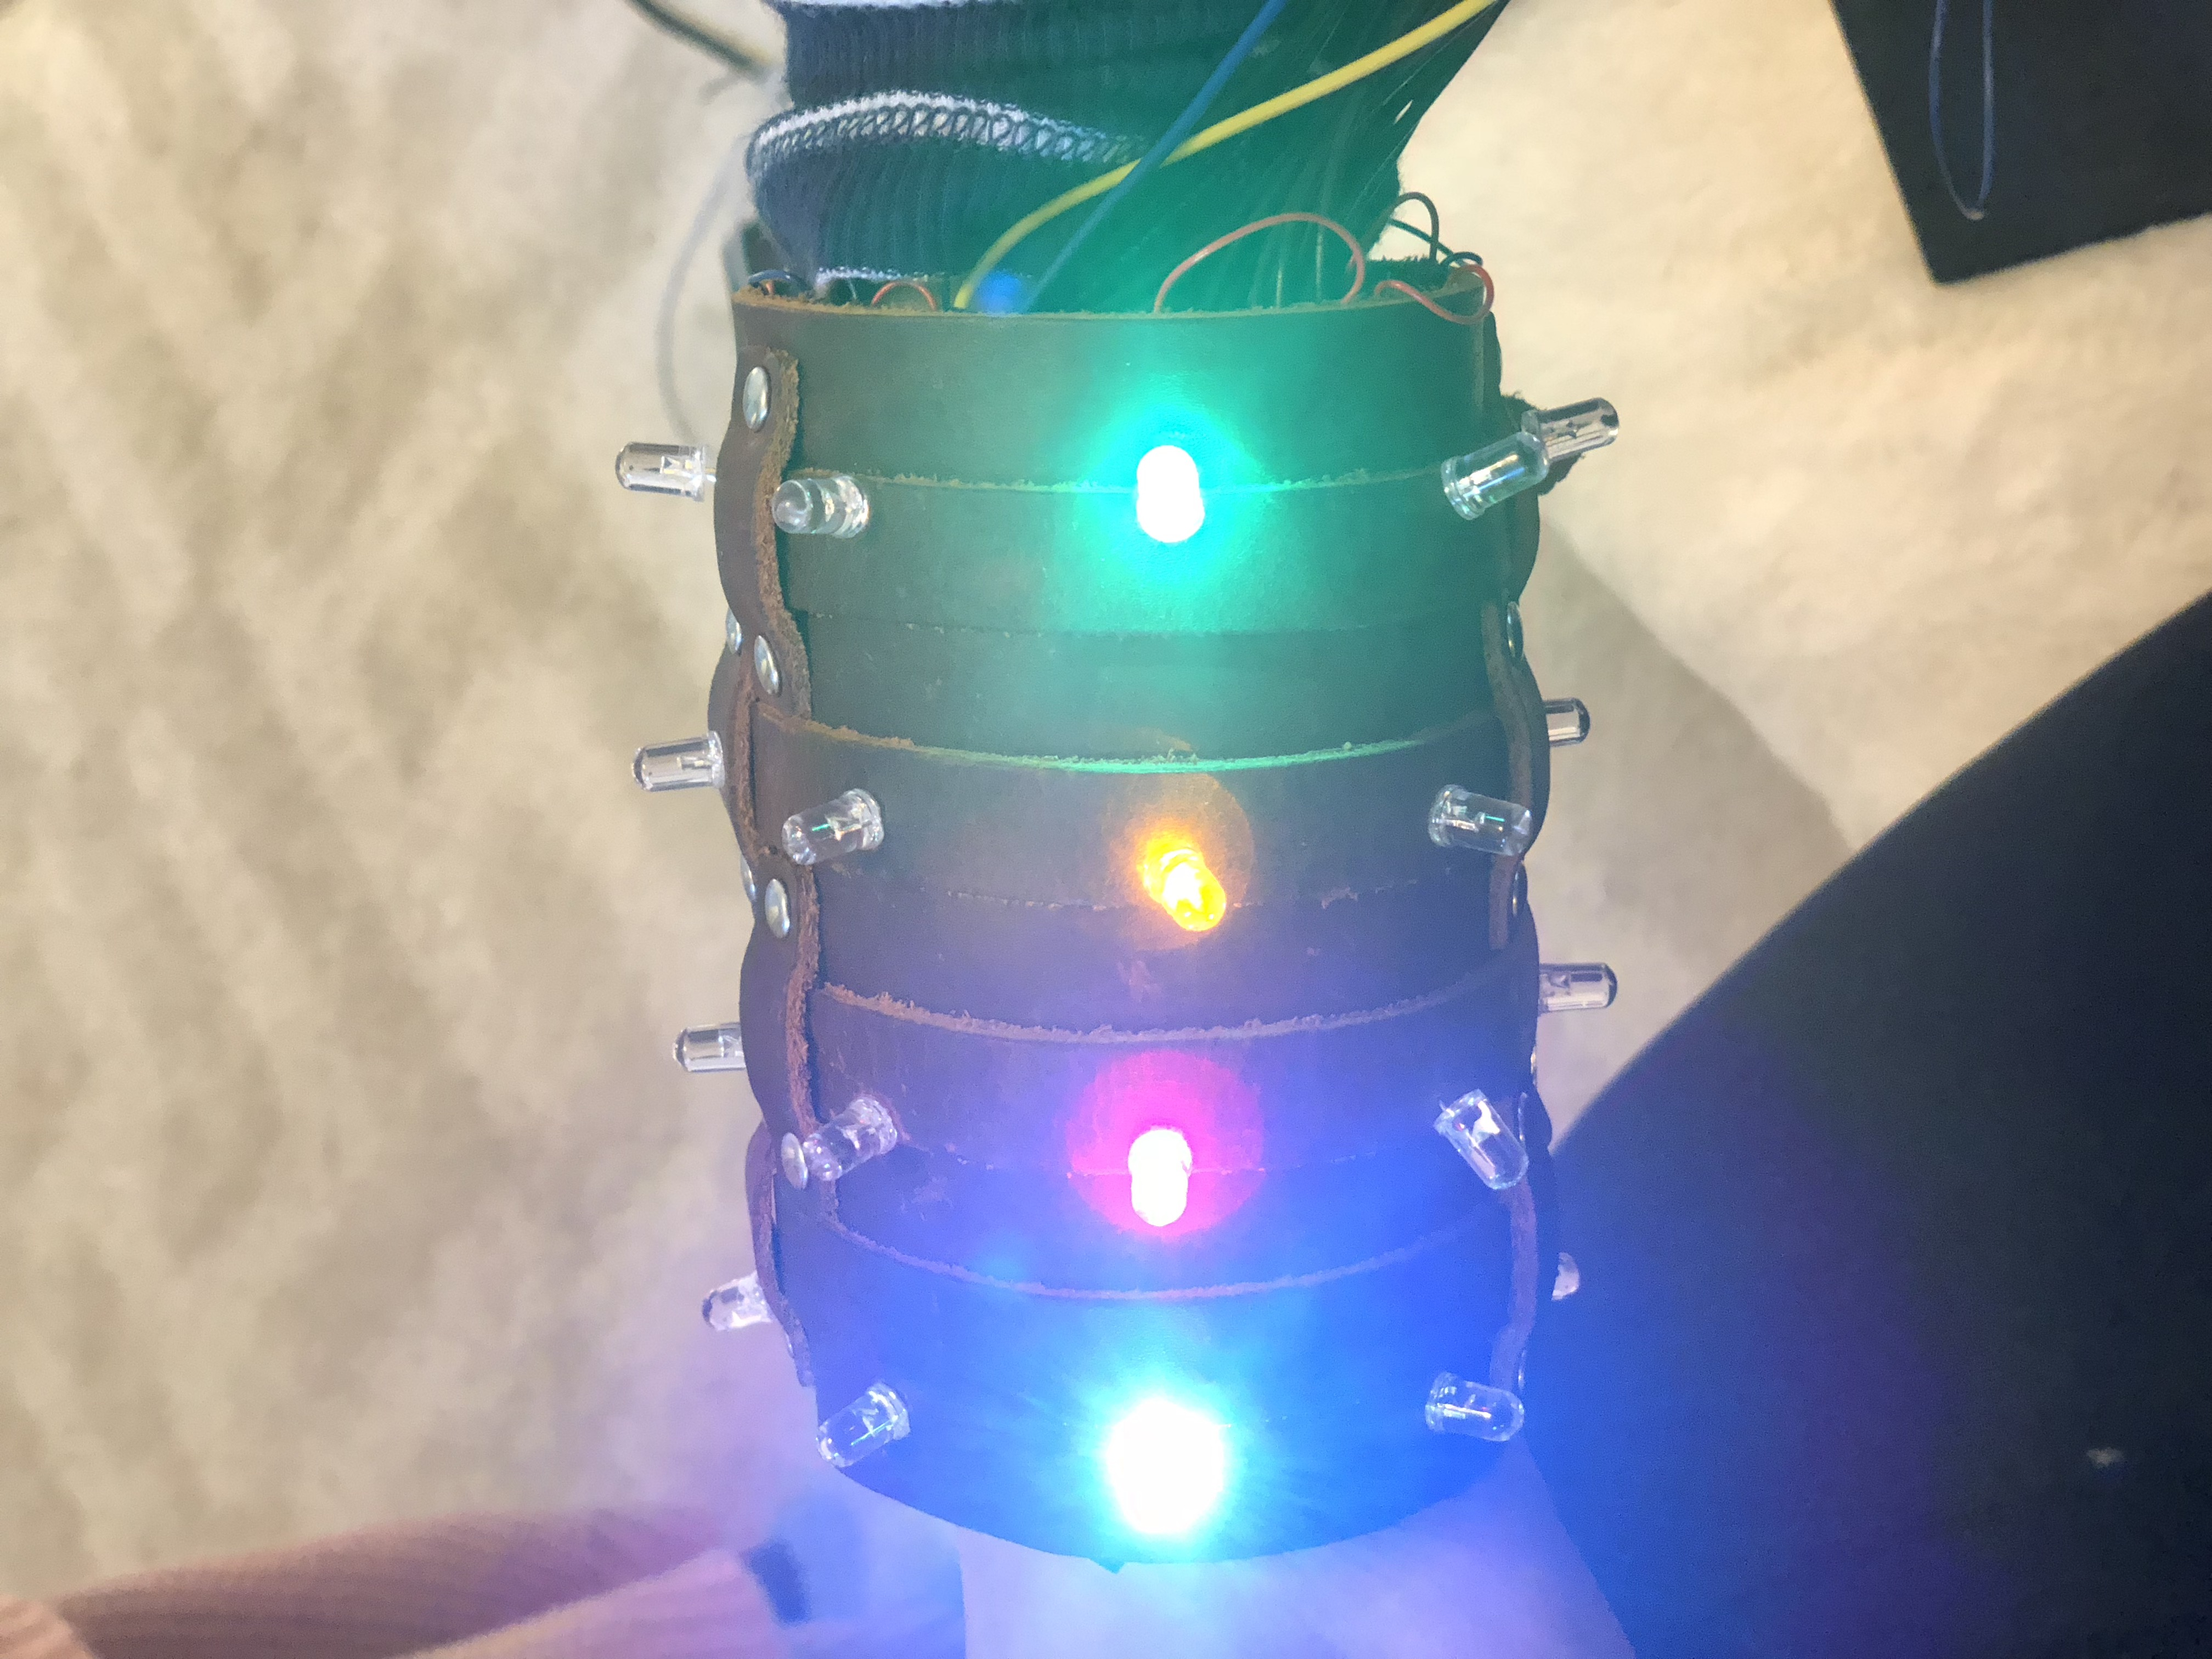
\includegraphics[width=4.0cm]{lit.JPG}}
%  \vspace{1.5cm}
  \centerline{(c) LED grid}\medskip
\end{minipage}
%
\caption{Pictures of the physical device.}
\label{figures}
%
\end{figure}
\end{center}



\section{RESULTS AND IMPROVEMENTS}
\label{sec:results}
We tested the device by blindfolding ourselves and equipping the wristband as shown in \textbf{Fig 3.} and camera then relying on the haptic feedback to guide us to the trash can. We turned the person testing the device around several times to disorient them before they set out to find the trash can. This way they had to only rely on the device to guide them to the trash can. It took some time, but the tester was able to find the trash can successfully. Towards the end of the demo, a couple of the haptic motors and LEDs got disconnected, so this means that we need to improve the overall robustness of our prototypes in the future. We also noted that a lot of the localization came from where the camera was with respect to the user. When her hand moved slightly too much to the left towards the end, only the right haptic motors set off, which would have indicated to the user that the trash can was to the right, however, she anticipated that she moved her hand and was still able to find the trash can. This is also something we would need to improve upon. The problem arises when the user moves too close to the camera. Since the trash can takes up the entire frame, even small changes in the way the camera is pointing could mislead the user into thinking that the trash can was far off in one direction. This can be solved by better communication to the user where the trash can is and how far away. In terms of image processing, another thing that could have been done better was to figure out better ways to process the image before feeding it into the model to get better results. Image processing can also be used for training purposes. Perhaps we could one day artificially create our own hidden colvolutional layers based off of filtering properties to help the network converge. In summary, our device was successful, but we have an incredibly long way to go and a major amount to learn. See \textbf{Appendix} for link to code.
\begin{figure}[ht]
    \centering
    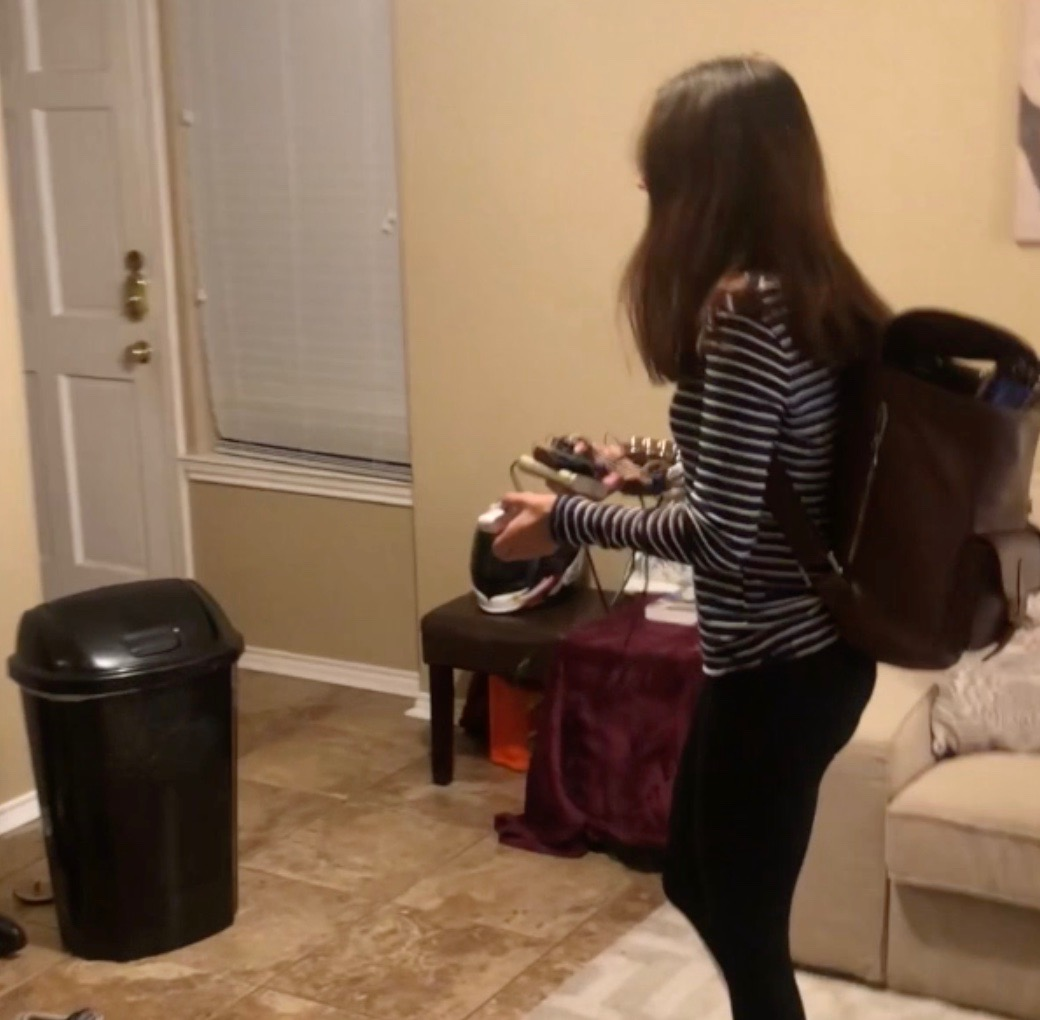
\includegraphics[width=.6\columnwidth]{demo.jpg}
    \caption{\label{fig:3} Us testing the device ourselves.}
\end{figure}


\section{CONCLUSION}
\label{sec:conclusion}

Currently, this device is used to locate public trash cans, but the concept is transferrable to anything in its domain such as maneuvering the blind away from hazardous obstacles, reading crucial public signs, and even experiencing a motion related performance such as a play. The list goes on. In final conclusion, image processing is a computational superpower, and we wanted to ultimately use that ability to even out the playing field by offering a new perspective to the blind and visually impaired. 

\section{ACKNOWLEDGMENTS}
\label{sec:ack}

Thank you, Dr. Alan C Bovik (Cockrell Family Regents Endowed Chair Professor, The University of Texas at Austin) for teaching us the concepts needed to implement this project. Also thank you to Rhanda Hasley, (President of the Dalla-Area Chapter of the National Federation for the Blind), for all of your advice.

\section{APPENDIX}
\label{sec:appendix}

\url{github.com/MKSwaminathan/Toad-Learns-Trash}

% To start a new column (but not a new page) and help balance the last-page

% column length use \vfill\pagebreak.
% -------------------------------------------------------------------------
%\vfill
%\pagebreak


% References should be produced using the bibtex program from suitable
% BiBTeX files (here: strings, refs, manuals). The IEEEbib.bst bibliography
% style file from IEEE produces unsorted bibliography list.
% -------------------------------------------------------------------------
\bibliographystyle{IEEEbib}
\bibliography{references}

\end{document}
